\documentclass[12pt]{article}
	\usepackage{mgates-letter}
	\definecolor{dark_blue} {rgb}{0., 0., 0.65}
	
	\usepackage{textcomp}
	\usepackage{mathrsfs}  % mathscr font
	\usepackage{boxedminipage}
	\usepackage{rotating}
	%\usepackage{natbib}
	\usepackage[colorlinks, filecolor=dark_blue, urlcolor=dark_blue, linkcolor=black, citecolor=black]{hyperref}
\begin{document}

\title{\LaTeX{} quick reference}
\author{Mark Gates}
\date{\today}
\maketitle

\noindent
\begin{minipage}{1.3in}
\href{http://creativecommons.org/licenses/by-sa/2.0/}{
\includegraphics[width=1.25in]{cc/by-sa.pdf}}
\end{minipage}
\begin{minipage}{5in}
This guide is available from
\href{http://web.eecs.utk.edu/~mgates3/}{http://web.eecs.utk.edu/${\sim}$mgates3/}
\\
Copyright \copyright 2007--2011 by Mark Gates.
\\
You may freely copy and modify this document under the
\href{http://creativecommons.org/licenses/by-sa/2.0/}{Creative Commons Attribution-ShareAlike license}.
When distributing modified versions, please include your Latex file.
\end{minipage}


\paragraph{Purpose.}

This document was initially made as a quick reference to all the
commands that I typically use, organized so I can understand it, with
examples and without clutter. It also includes many shortcuts that I
have defined in my mgates.sty file. It is not intended to be exhaustive,
nor overly descriptive. Most of the general \LaTeX commands can be found
in the \emph{Not So Short Introduction to \LaTeXe} \cite{NotSoShort};
most of the math in the \emph{Short Math Guide to \LaTeX}
\cite{AMSShortGuide}; most of the bibliography information in the BibTeX
tutorial \cite{Markey05} and the natbib documentation \cite{Daly06}.

I also wrote a separate Latex fonts guide.


% ----------------------------------------
\newpage
\setcounter{tocdepth}{2}
\tableofcontents

% set these after the TOC
\setlength{\parindent}{0em}
\setlength{\parskip}{1em}


% ----------------------------------------
\newpage
\section{Commands}

\subsection{Document structure}

\verb+\documentclass[+\emph{options}\verb+]{+\emph{class}\verb+}+

\textbf{Common classes} \\
\begin{tabular}{@{}ll}
article  &  articles without chapters      \\
proc     &  proceedings, based on article  \\
minimal  &  minimal formatting             \\
report   &  reports with chapters          \\
book     &  real books                     \\
\end{tabular}

\textbf{Common options} \\
\begin{tabular}{@{}ll}
10pt, 11pt, 12pt           &  main font size                              \\
a4paper, letterpaper, ...  &  paper size                                  \\
fleqn                      &  equations left-aligned instead of centered  \\
leqno                      &  equation numbers on left instead of right   \\
titlepage, notitlepage     &  start new page after title                  \\
onecolumn, twocolumn       &  one or two columns                          \\
twoside, oneside           &                                              \\
landscape                  &  paper orientation                           \\
openright, openany         &  chapters begin on right page, or any page   \\
\end{tabular}

\subsubsection*{Preamble}

\verb+\usepackage[+\emph{options}\verb+]{+\emph{package}\verb+}+

\verb+\includeonly{+\emph{filenames}\verb+}+ \\
skip \verb+\include+ with listed files

\subsubsection*{Document}

\verb+\begin{document}+

\verb+\include{+\emph{filename}\verb+}+ \\
start new page with contents of file

\verb+\input{+\emph{filename}\verb+}+ \\
include contents of file, without starting a new page

\verb+\end{document}+


% ----------------------------------------
\newpage
\subsection{Page format}

\verb+\pagestyle{ plain | headings | empty }+   \\
\begin{tabular}{@{}ll}
plain     &  page number in footer              \\
headings  &  page number and chapter in header  \\
empty     &  no header or footer                \\
\end{tabular}


\verb+\thispagestyle{ plain | headings | empty }+ \\
override \verb+\pagestyle+ on a single page

\begin{verbatim}
% set 1" margins on 8.5" x 11" paper
% top left is measured from 1", 1"
\topmargin       0in
\oddsidemargin   0in
\evensidemargin  0in
\headheight      0in
\headsep         0in
\topskip         0in
\textheight      9in
\textwidth       6.5in

% set these after the TOC
\setlength{\parindent}{0em}
\setlength{\parskip}{1em}

\setlength\arraycolsep{2pt}
\end{verbatim}


% ----------------------------------------
\newpage
\subsection{Chapters and Sections}

\verb+\title{...}+ \\
\verb+\author{John Doe \and Jane Doe}+ \\
\verb+\date{\today}+ \\
\verb+\maketitle+

\verb+\frontmatter  %+ (book only) starts roman numeral page numbering, unnumbered sections

\verb+\setcounter{tocdepth}{1}  %+ whether to display sub- or subsubsections in toc \\
\verb+\tableofcontents+

\verb+\mainmatter   %+ (book only) starts arabic page \& section numbering

\verb+\part{...}+  \\          
\verb+\chapter{...}            \chapter*{...}        %+ (book only) \\
\verb+\section{...}            \section*{...}+        \\
\verb+\subsection{...}         \subsection*{...}+     \\
\verb+\subsubsection{...}      \subsubsection*{...}+  \\
\verb+\paragraph{...}          \paragraph*{...}+      \\
\verb+\subparagraph{...}       \subparagraph*{...}+

\verb+\appendix     %+ (book only) starts alphabetic section numbering

\verb+\backmatter+

* Starred versions are unnumbered and not in the table of contents.

Examples:

\begin{boxedminipage}{6.5in}
\section*{1 \quad section}

\subsection*{1.1 \quad subsection}

\subsubsection*{1.1.1 \quad subsubsection}

\paragraph{paragraph} Run-in paragraph header. Lorem ipsum dolar
blah blah blah blah blah blah blah blah blah blah blah blah blah blah

\subparagraph{subparagraph} Run-in paragraph header. Lorem ipsum dolar
blah blah blah blah blah blah blah blah blah blah blah blah blah blah
\end{boxedminipage}


% ----------------------------------------
\newpage
\subsection{Fonts}

\textbf{Font sizes} \\
\begin{tabular}{@{}lllll}
\multicolumn{2}{@{}l}{Point size}
        &  Latex cmd             &  User-defined *     &  Sample \\
\hline
 5 &  6 &  \verb+\tiny+          &  \verb+\xxxsmall+   &  \xxxsmall {the quick brown fox} \\
 7 &  8 &  \verb+\scriptsize+    &  \verb+\xxsmall+    &  \xxsmall  {the quick brown fox} \\
 8 & 10 &  \verb+\footnotesize+  &  \verb+\xsmall+     &  \xsmall   {the quick brown fox} \\
 9 & 11 &  \verb+\small+         &  \verb+\small+      &  \small    {the quick brown fox} \\
\textbf{10} & \textbf{12}
        &  \verb+\normal+        &  \verb+\normal+     &  \normal   {the quick brown fox} \\
\hline
12 & 14 &  \verb+\large+         &  \verb+\large+      &  \large    {the quick brown fox} \\
14 & 17 &  \verb+\Large+         &  \verb+\xlarge+     &  \xlarge   {the quick brown fox} \\
17 & 20 &  \verb+\LARGE+         &  \verb+\xxlarge+    &  \xxlarge  {the quick brown fox} \\
20 & 25 &  \verb+\huge+          &  \verb+\xxxlarge+   &  \xxxlarge {the quick brown fox} \\
25 & 25 &  \verb+\Huge+          &  \verb+\xxxxlarge+  &  \xxxxlarge{the quick brown fox} \\
\end{tabular}

* see mgates.sty file

\textbf{Fonts} \\
\begin{tabular}{@{}ll}
Command             &  Sample                \\
\hline
\verb+\textrm+      &  \textrm{roman}        \\
\verb+\textsf+      &  \textsf{sans serif}   \\
\verb+\texttt+      &  \texttt{typewriter}   \\
\verb+\textup+      &  \textup{upright}      \\
\verb+\textsl+      &  \textsl{slanted}      \\
\verb+\emph+        &  \emph{emphasized}     \\
\verb+\underline+   &  \underline{underline} \\
\verb+\textit+      &  \textit{italic}       \\
\verb+\textmd+      &  \textmd{medium}       \\
\verb+\textbf+      &  \textbf{bold font}    \\
\verb+\textsc+      &  \textsc{Small Caps}   \\
\verb+\textnormal+  &  \textnormal{normal}   \\
\end{tabular}

In math mode (e.g. inside \$...\$), use the math fonts listed in the
math section.


% ----------------------------------------
\newpage
\subsection{Reserved characters}

\begin{tabular}{@{}lll}
Char      &  Special meaning    &  Command      \\
\hline
\verb+#+  &  ?                  &  \verb+\#+    \\
\verb+$+  &  math mode          &  \verb+\$+    \\
\verb+%+  &  comment            &  \verb+\%+    \\
\verb+^+  &  math superscript   &  \verb+\^{}+  \\
\verb+&+  &  tab stop           &  \verb+\&+    \\
\verb+_+  &  math subscript     &  \verb+\_+    \\
\verb+{+  &  start parameter    &  \verb+\{+    \\
\verb+}+  &  end parameter      &  \verb+\+     \\
\verb+~+  &  nonbreaking space  &  \verb+\~{}+  \\
\verb+\+  &  start command      &  \verb+$\backslash$+ \\
\end{tabular}

These can also be typed in the verbatim environment or with \verb+\verb+.


% ----------------------------------------
\subsection{Special characters}

\begin{tabular}{@{}ll|ll|ll}
Symbol           &  Command                 &
Symbol           &  Command                 &
Symbol           &  Command
\\
\hline
``               &  \verb+``+               &
"                &  \verb+"+ or \verb+''+   &
\\
`                &  \verb+`+                &
'                &  \verb+'+                &
\\
in-law           &  \verb+in-law+           &
13--67 (en)      &  \verb+13--67+           &
yes---no (em)    &  \verb+yes---no+
\\
yes \ldots no    &  \verb+yes \ldots no+    &
?`No?            &  \verb+?`No?+            &
!`No!            &  \verb+!`No!+
\\
\dag             &  \verb+\dag+             &
\ddag            &  \verb+\ddag+            &
\\
\S               &  \verb+\S+               &
\P               &  \verb+\P+               &
\\
\copyright       &  \verb+\copyright+       &
\textregistered  &  \verb+\textregistered+  &
\\
\pounds          &  \verb+\pounds+          &
\texteuro        &  \verb+\texteuro+ *      &
\\
\end{tabular}

* in textcomp package


% ----------------------------------------
\newpage
\subsection{Accented characters}

\begin{tabular}{@{}ll|ll|ll|ll}
Char  &  Command      &
Char  &  Command      &
Char  &  Command      &
Char  &  Command
\\
\hline
\`o   &  \verb+\`o+   &
\'o   &  \verb+\'o+   &
\^o   &  \verb+\^o+   &
\~o   &  \verb+\~o+
\\
\=o   &  \verb+\=o+   &
\.o   &  \verb+\.o+   &
\"o   &  \verb+\"o+   &
\c c  &  \verb+\c+ c
\\
\u o  &  \verb+\u o+  &
\v o  &  \verb+\v o+  &
\H o  &  \verb+\H o+  &
\\
\d o  &  \verb+\d o+  &
\b o  &  \verb+\b o+  &
\t oo &  \verb+\t oo+ &
\\
\hline
\oe   &  \verb+\oe+   &
\OE   &  \verb+\OE+   &
\ae   &  \verb+\ae+   &
\AE   &  \verb+\AE+
\\
\aa   &  \verb+\aa+   &
\AA   &  \verb+\AA+   &
\\
\o    &  \verb+\o+    &
\O    &  \verb+\O+    &
\l    &  \verb+\l+    &
\L    &  \verb+\L+
\\
\end{tabular}

The first 4 lines can be applied to appropriate characters. \\
To put accent over \emph{i} or \emph{j}, use \verb+\i+ (\i) or \verb+\j+ (\j).


% ----------------------------------------
\subsection{Special spaces}

\begin{tabular}{@{}llll}
Command        &  Size         &  1 space   &  10 spaces               \\
\hline
\verb+\,+      &  $3/8$ quad   &  (\,)      &  [\,\,\,\,\,\,\,\,\,\,]  \\
\verb+\:+      &  $4/8$ quad   &  (\:)      &  [\:\:\:\:\:\:\:\:\:\:]  \\
\verb+\;+      &  $5/8$ quad   &  (\;)      &  [\;\;\;\;\;\;\;\;\;\;]  \\
\verb*+\ +     &  en? space    &  (\ )      &  [\ \ \ \ \ \ \ \ \ \ ]  \\
\verb+\quad+   &  em  space    &  (\quad)   &  [\quad\quad\quad\quad\quad\quad\quad\quad\quad\quad]  \\
\verb+\qquad+  &  $2$ quad     &  (\qquad)  &  [\qquad\qquad\qquad\qquad\qquad\qquad\qquad\qquad\qquad\qquad]  \\
\verb+\!+      &  $-3/8$ quad  &  (\!)      &  [\!\!\!\!\!\!\!\!\!\!]  \\
\end{tabular}

In math mode, \verb+phantom+ reserves space for text without printing it,
for example \\
\begin{minipage}{3in}
\begin{align*}
	x_1 \phantom{+ x_2} + x_3 = 2,  \\
	x_1 + x_2 \phantom{+ x_3} = 5,  \\
	x_1 + x_2 + x_3 = 7.
\end{align*}
\end{minipage}
\qquad
\begin{minipage}{3in}
\begin{verbatim}
	
	
	x_1 \phantom{+ x_2} + x_3 = 2,  \\
	x_1 + x_2 \phantom{+ x_3} = 5,  \\
	x_1 + x_2 + x_3 = 7.
\end{verbatim}
\end{minipage}


% ----------------------------------------
\subsection{Special phrases}

\begin{tabular}{@{}ll}
Command         &  Sample  \\
\hline
\verb+\today+   &  \today  \\
\verb+\TeX+     &  \TeX    \\
\verb+\LaTeX+   &  \LaTeX  \\
\verb+\LaTeXe+  &  \LaTeXe \\
\end{tabular}


% ----------------------------------------
\newpage
\subsection{Line and page breaks}

\verb+\\+ or \verb+\newline+ \\
line break, without new paragraph. \verb+\\*+ also prohibts page break.

\verb+\linebreak[+\emph{n}\verb+]+ \\
\verb+\nolinebreak[+\emph{n}\verb+]+ \\
line break, keeping line justified.
$n$ ranges from 0 to 4 (most insistent).

\begin{boxedminipage}{\textwidth}
For example, here is a paragraph with a newline in it, lorem ipsum dolar
blah blah blah blah blah blah blah blah blah blah blah blah blah blah blah,
\verb+\newline+. \\
It also has a linebreak in it for comparison, lorem ipsum dolar 
blah blah blah blah blah blah blah blah blah blah blah blah blah blah blah,
\verb+\linebreak[4]+. \linebreak[4]
Notice the difference in justification. Using \verb+\linebreak+ can
cause ``underfull hbox'' warnings.
\end{boxedminipage}

\verb+\newpage+ \\
page break

\verb+\pagebreak[+\emph{n}\verb+]+ \\
\verb+\nopagebreak[+\emph{n}\verb+]+ \\
page break, keeping line justified.
$n$ ranges from 0 to 4 (most insistent).

\verb+\hyphenation{ fortran hy-phen-a-tion }+ \\
list of words and where they may be hyphenated (in preamble).

\verb+\-+ \\
where a word may be hyphenated (in text).
Example: \verb+su\-per\-scal\-ar+

\verb*+\ +  space not to enlarge \\
\verb+~+   space not to enlarge or line break \\
``Mr.\ Smith''  (\verb+Mr.\ Smith+)  or \\
``Mr.~Smith''   (\verb+Mr.~Smith+)   instead of \\
``Mr. Smith''   (\verb+Mr. Smith+)

\verb+\@+  between capital letter and punctuation that really does end a sentance \\
``\ldots FORTRAN\@. But\ldots''  (\verb+FORTRAN\@. But+)  instead of \\
``\ldots FORTRAN. But\ldots''    (\verb+FORTRAN. But+)


% ----------------------------------------
\newpage
\subsection{References, citations, footnotes}
\label{references}

\verb+\label{+\emph{name}\verb+}+ assigns a unique name to an
equation, figure, table, or section. For figures and tables, label must
be after the caption.

\verb+\eqref{+\emph{name}\verb+}+ inserts reference to the labeled
equation; equivalent to \verb+(\ref{+\emph{name}\verb+})+.

\verb+\ref{+\emph{name}\verb+}+ inserts reference to the label.
You must add the descriptive text such as ``figure.''

\verb+\pageref{+\emph{name}\verb+}+ inserts page number of the label.

\verb+\cite{+\emph{name}\verb+}+ inserts reference to bibliography
citation. Name is assigned by \verb+bibitem+, not \verb+label+.

\verb+\footnote{+\emph{text}\verb+}+ generates a footnote.

See also equation numbering on page \pageref{equation-numbering}.


% ----------------------------------------
\subsection{Hyperlinks}

\verb+\usepackage[+\emph{options}\verb+]{hyperref}+
\\
\verb+\usepackage[colorlinks, urlcolor=blue, linkcolor=black]{hyperref}+

To color links, use the \verb+colorlinks+ option. To override default colors, specify \\
\begin{tabular}{@{}lll}
linkcolor  &  red      &  internal links (sections, pages, etc.)  \\
citecolor  &  green    &  citation links (bibliography)           \\
filecolor  &  magenta  &  file links                              \\
urlcolor   &  cyan     &  URL links (mail, web)                   \\
\end{tabular}

 \verb+\href{+\emph{url}\verb+}{+\emph{text}\verb+}+ \\
 \verb+\href{http://www.ctan.org/}{CTAN}+
\qquad \href{http://www.ctan.org/}{CTAN}

 \verb+\href{mailto:noone@example.com}{noone@example.com}+
\qquad \href{mailto:noone@example.com}{noone@example.com}


% ----------------------------------------
\newpage
\section{Environments}

\subsection{Text alignment}

\begin{boxedminipage}[t]{3in}
	\begin{flushleft}
	this paragraph is \\
	flush left.
	\end{flushleft}
\end{boxedminipage}
\qquad
\begin{minipage}[t]{3in}
\begin{verbatim}
	\begin{flushleft}
	this paragraph \\
	is flush left.
	\end{flushleft}
\end{verbatim}
\end{minipage}

\begin{boxedminipage}[t]{3in}
	\begin{flushright}
	this paragraph is \\
	flush right.
	\end{flushright}
\end{boxedminipage}
\qquad
\begin{minipage}[t]{3in}
\begin{verbatim}
	\begin{flushright}
	this paragraph \\
	is flush right.
	\end{flushright}
\end{verbatim}
\end{minipage}

\begin{boxedminipage}[t]{3in}
	\begin{center}
	this paragraph is \\
	centered.
	\end{center}
\end{boxedminipage}
\qquad
\begin{minipage}[t]{3in}
\begin{verbatim}
	\begin{center}
	this paragraph \\
	is centered.
	\end{center}
\end{verbatim}
\end{minipage}


% ----------------------------------------
\subsection{Boxes}

Only minipage is an environment, but these are all related.

\verb+\mbox{...}+ \\
\verb+\makebox[+\emph{width}\verb+][t|b|c]{...}+ \\
groups items in a box. Everything must be on one line (?).

\verb+\fbox{...}+ \\
\verb+\framebox[+\emph{width}\verb+][t|b|c]{...}+ \\
framed box. Everything must be on one line (?).

\verb+\parbox[t|b|c]{+\emph{width}\verb+}{...}+ \\
paragraph box that wraps text.

\verb+\begin{minipage}[t|b|c]{+\emph{width}\verb+} ... \end{minipage}+ \\
minipage box, similar to parbox but can contain almost anything.

\verb+\begin{boxedminipage}[t|b|c]{+\emph{width}\verb+} ... \end{boxedminipage}+ \\
with \verb+\usepackage{boxedminipage}+.

\verb+\rule{+\emph{width}\verb+}{+\emph{height}\verb+}+

\verb+\raisebox+

page and other parameters to tweak


% ----------------------------------------
\newpage
\subsection{Block quotes}

\begin{boxedminipage}[t]{3in}
	Martin Luther King Jr. said,
	\begin{quote}
	I have a dream that someday\ldots
	\end{quote}
\end{boxedminipage}
\qquad
\begin{minipage}[t]{3in}
\begin{verbatim}
	Martin Luther King Jr. said,
	\begin{quote}
	I have a dream that someday\ldots
	\end{quote}
\end{verbatim}
\end{minipage}

For multiple paragraph quotations, use \verb+quotation+ instead of
\verb+quote+, to indent the first line of each paragraph.


\subsection{Verse}

Reverse indents if line wraps.

\begin{boxedminipage}[t]{3in}
	\textbf{Humpty Dumpty}
	\begin{verse}
	Humpty Dumpty sat on a wall:\\
	Humpty Dumpty had a great fall.\\
	All the King's horses and all the King's men\\
	Couldn't put Humpty together again.
	\end{verse}
\end{boxedminipage}
\qquad
\begin{minipage}[t]{3in}
\begin{verbatim}
	\textbf{Humpty Dumpty}
	\begin{verse}
	Humpty Dumpty sat on a wall:\\
	Humpty Dumpty had a great fall.\\
	All the King's horses and all the
	King's men\\
	Couldn't put Humpty together again.
	\end{verse}
\end{verbatim}
\end{minipage}



% ----------------------------------------
\subsection{Verbatim}

\verb+verbatim+ reproduces text exactly as you type it,
not interpretting any characters or commands. It was used
here for all the LaTeX code listings.

% note \end{verbatim} obviously can't be
% inside \begin{verbatim}...\end{verbatim}
\verb+\begin{verbatim}+ \\
\verb+text can include special characters # $ < + \\
\verb+and \textbf{commands}.+ \\
\verb+\end{verbatim}+

\verb|\verb+text+| \\
where the delimiter `+' is any character except letters, *, and space.

Adding a star highlights spaces. \\
\verb+\begin{verbatim*} ... \end{verbatim*}+ \\
\verb|\verb*+text with spaces+|  \qquad \verb*+text with spaces+


% ----------------------------------------
\newpage
\subsection{Lists}

\begin{boxedminipage}[t]{3in}
	\begin{enumerate}
	\item One
	\item[3.] Two (with special number)
	\item Three
	\end{enumerate}
\end{boxedminipage}
\qquad
\begin{minipage}[t]{3in}
\begin{verbatim}
	\begin{enumerate}
	\item One
	\item[3.] Two (with special number)
	\item Three
	\end{enumerate}
\end{verbatim}
\end{minipage}

\begin{boxedminipage}[t]{3in}
	\begin{itemize}
	\item One
	\item[-] Two (with special bullet)
	\end{itemize}
\end{boxedminipage}
\qquad
\begin{minipage}[t]{3in}
	\begin{verbatim}
	\begin{itemize}
	\item One
	\item[-] Two (with special bullet)
	\end{itemize}
\end{verbatim}
\end{minipage}

\begin{boxedminipage}[t]{3in}
	\begin{description}
	\item[One] Description of one
	\item[Two] Description of two
	\end{description}
\end{boxedminipage}
\qquad
\begin{minipage}[t]{3in}
\begin{verbatim}
	\begin{description}
	\item[One] Description of one
	\item[Two] Description of two
	\end{description}
\end{verbatim}
\end{minipage}


% ----------------------------------------
\subsection{Tables (tabular)}

\begin{boxedminipage}[t]{3in}
	\begin{tabular}{l|ll}
	col1  &  col2  &  col3 \\
	\hline
	col1  &  col2  &  col3 \\
	col1  &  col2  &  col3
	\end{tabular}
\end{boxedminipage}
\qquad
\begin{minipage}[t]{3in}
	\vspace{-24pt}
	\begin{verbatim}
	\begin{tabular}{l|ll}
	col1  &  col2  &  col3 \\
	\hline
	col1  &  col2  &  col3 \\
	col1  &  col2  &  col3 \\
	\end{tabular}
	\end{verbatim}
\end{minipage}

In general: \\
\verb+\begin{tabular}[t|b|c]{+\emph{column spec}\verb+}+ \\
\verb+col1  &  col2  &  ...  &  coln \\+ \\
\verb+col1  &  col2  &  ...  &  coln \\+ \\
\verb+\end{tabular}+

In \emph{column spec}, for each column use \verb+l+, \verb+r+, \verb+c+
for a left, right, or centered column, \verb+p{+\emph{width}\verb+}+ for
a column of given width that wraps text. Use \verb+|+ (pipe) for a
vertical line between columns. Use \verb+@{...}+ to specify the
delimiter between columns. An empty \verb+@{}+ deletes the gutter or
left indent.

Between lines, use \verb+\hline+ for a horizontal line.

Use \verb+\multicolumn{+\emph{n}\verb+}{+\emph{column spec}\verb+}{+\emph{text}\verb+}+
to have text span multiple columns.


% ----------------------------------------
\newpage
\subsection{Figures and Tables}

A figure typically includes 1 or more graphics. Example:

\begin{figure}[h]
	\begin{boxedminipage}{3in}
		    \centering
		    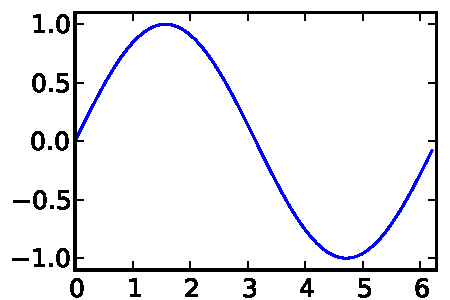
\includegraphics[scale=0.8]{sine}
		    \caption{$\sin(x)$}
		    \label{sine}
	\end{boxedminipage}
	\qquad
	\begin{minipage}{3in}
		\begin{verbatim}
		\begin{figure}[h]
		    \centering
		    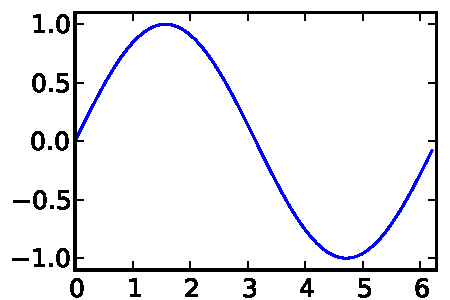
\includegraphics[scale=0.8]{sine}
		    \caption{$\sin(x)$}
		    \label{sine}
		\end{figure}
		\end{verbatim}
	\end{minipage}
\end{figure}

A table typically includes a tabular environment; see previous section.
Example:

\begin{table}[h]
	\begin{boxedminipage}{3in}
		    \centering
		    \begin{tabular}{ccc}
		          &  sales   &  growth  \\
		    2000  &  10,000  &  15\%  \\
		    2001  &  12,000  &  20\%  \\
		    \end{tabular}
		    \caption{Sales growth}
		    \label{sales-growth}
	\end{boxedminipage}
	\qquad
	\begin{minipage}{3in}
		\begin{verbatim}
		\begin{table}[h]
		    \centering
		    \begin{tabular}{ccc}
		          &  sales   &  growth  \\
		    2000  &  10,000  &  15\%  \\
		    2001  &  12,000  &  20\%  \\
		    \end{tabular}
		    \caption{Sales growth}
		    \label{sales-growth}
		\end{table}
		\end{verbatim}
	\end{minipage}
\end{table}

\verb+figure+ and \verb+table+ take an optional placement specifier: \\
\begin{tabular}{@{}ll}
\verb+h+  &  \emph{here} in the text  \\
\verb+t+  &  \emph{top} of a page     \\
\verb+b+  &  \emph{bottom} of a page  \\
\verb+p+  &  on a special \emph{page} of only floats  \\
\verb+!+  &  be insistent             \\
\end{tabular}

To use \verb+includegraphics+, include
\verb+\usepackage[+\emph{driver}\verb+]{graphicx}+ 
in the preamble. The \emph{driver} should normally be omitted; if necesary,
it is \verb+dvips+ for latex
and \verb+pdftex+ for pdflatex. Files must be eps for dvips, while
pdftex takes pdf, jpg, tif, or png. It's convenient to leave off the
extension; latex/pdflatex will look for the appropriate file. (In this
example, spring.pdf or spring.eps.) Since many journals want eps
files instead of pdf files, I often generate eps files first, then
convert them to pdf using epstopdf.

\verb+includegraphics+ options \\
\begin{tabular}{@{}ll}
\verb+width=+\emph{width}    &  scale to width, maintaining aspect ratio if no height  \\
\verb+height=+\emph{height}  &  scale to height, maintaining aspect ratio if no width  \\
\verb+angle=+\emph{degrees}  &  rotate counterclockwise                                \\
\verb+scale=+\emph{scale}    &  resize image by scalar value                           \\
\end{tabular}


% ----------------------------------------
\newpage
\section{Math}

Surround inline equations with dollar signs, for example \verb+$x=2$+
produces $x=2$. For equations in their own block, use one of the
environments below. For unnumbered equations append a * star to the
environment name. As a shortcut for unnumbered equations, \verb+\[...\]+
is the same as \verb+\begin{equation*}...\end{equation*}+.

\noindent
\rule{6.5in}{0.5pt}

\noindent
\begin{minipage}[t]{3.125in}
\verb+equation+ sets a single equation \eqref{x1}.
%
\begin{equation} \label{x1}
	x = a + b.
\end{equation}
%
\verb+gather+ sets multiple equations (\ref{x2},\ref{y2}), centered on
each other.
%
\begin{gather}
	x = a + b,         \label{x2} \\
	y = c + d + e + f. \label{y2} 
\end{gather}
%
\verb+align+ sets multiple equations (\ref{x3},\ref{y3}), aligned
typically on $=$ sign.
%
\begin{align}
	x &= a + b,         \label{x3} \\
	y &= c + d + e + f, \label{y3}
\end{align}
%
\verb+multline+ splits a long equation
\eqref{x6} over multiple lines, distributing the space.
%
\begin{multline} \label{x6}
	x = a + b + c + d + e + f\\
		+ g + h + i + j + k. \\
		+ l + m + n.
\end{multline}
%
\verb+split+ splits a long equation \eqref{x5} over multiple
lines, aligning it. Use inside equation, align, or gather.
%
\begin{equation}
\begin{split} \label{x5}
	x &= a + b      \\
	  &= c + d + e.
\end{split}
\end{equation}
%
\verb+subequations+ assigns all enclosed equations subordinate equation
numbering, so (\ref{x4},\ref{y4}) are parts of \eqref{group4}.
%
\begin{subequations} \label{group4}
\begin{align}
	x &= a + b,         \label{x4} \\
	y &= c + d + e + f. \label{y4}
\end{align}
\end{subequations}
\end{minipage}
\hspace{1em}
\begin{minipage}[t]{3.125in}
\begin{verbatim}
\begin{equation} \label{x1}
	x = a + b.
\end{equation}
\end{verbatim}
\vspace{-16pt}
\begin{verbatim}
\begin{gather}
	x = a + b,         \label{x2} \\
	y = c + d + e + f. \label{y2} 
\end{gather}
\end{verbatim}
\vspace{-0pt}
\begin{verbatim}
\begin{align}
	x &= a + b,         \label{x3} \\
	y &= c + d + e + f, \label{y3}
\end{align}
\end{verbatim}
\vspace{2pt}
\begin{verbatim}
\begin{multline} \label{x6}
	x = a + b + c + d + e + f \\
	  + g + h + i + j + k. \\
	  + l + m + n.
\end{multline}
\end{verbatim}
\vspace{6pt}
\begin{verbatim}
\begin{equation}
\begin{split} \label{x5}
	x &= a + b      \\
	  &= c + d + e.
\end{split}
\end{equation}
\end{verbatim}
\vspace{-14pt}
\begin{verbatim}
\begin{subequations} \label{group4}
\begin{align}
	x &= a + b,         \label{x4} \\
	y &= c + d + e + f. \label{y4}
\end{align}
\end{subequations}
\end{verbatim}
\end{minipage}

\newpage

\noindent
\begin{minipage}[t]{3in}
\verb+align+ can also have several columns of equations or descriptions.
The \verb+intertext+ command is useful to insert text while preserving
alignment.
\begin{align*}
	x &= 1, & y &= 2, && \text{initialize}
	\\
	z &= 3, & w &= 4,
\intertext{some more text, and}
	a &= 5, & b &= 5.
\end{align*}
%
The non-AMS command for aligning equations is \verb+eqnarray+, but it
produces rather poor spacing and is \emph{not recommended}.
%
\begin{eqnarray}
	x &=& a + b,         \label{x7} \\
	y &=& c + d + e + f. \label{y7}
\end{eqnarray}
%
\end{minipage}
\hspace{1em}
\begin{minipage}[t]{3in}
\begin{verbatim}
\begin{align*}
	x &= 1, & y &= 2, && \text{initialize}
	\\
	z &= 3, & w &= 4,
\intertext{some more text, and}
	a &= 5, & b &= 5.
\end{align*}
\end{verbatim}
\vspace{46pt}
\begin{verbatim}
\begin{eqnarray}
	x &=& a + b,         \label{x7} \\
	y &=& c + d + e + f. \label{y7}
\end{eqnarray}
\end{verbatim}
\end{minipage}

\noindent
\rule{6.5in}{0.5pt}


% ----------------------------------------
\subsection{Equation numbering}
\label{equation-numbering}

\verb+\label{+\emph{name}\verb+}+ assigns a unique name to an
equation.

\verb+\eqref{+\emph{name}\verb+}+ generates reference to equation;
equivalent to \verb+(\ref{+\emph{name}\verb+})+

For \verb+subequations+, both the whole group and individial equations
can have labels.

To get equation numbers of form $m.n$ where $m$ is the section number
and $n$ is the equation number within section, use
\verb+\numberwithin{equation}{section}+ in preamble.

See also references on page \pageref{references}.


% ----------
\subsection{Sub/superscripts}

Subscripts are done with \_ underbar, like \verb+x_{1}+ for $x_1$.
\\
Superscripts are done with \^{} caret, like \verb+x^{1}+ for $x^1$.
\\
Use braces for double sub/superscripts, like
\verb+{B^a}^T+ for ${B^a}^T$ or \verb+\int_{x_1}+ for $\int_{x_1}$.


% ----------
\subsection{Fractions and binomial coefficient}

\verb+\frac{+\emph{numerator}\verb+}{+\emph{denominator}\verb+}+
makes fractions in either display or text style, depending on context.
\\
\verb+\dfrac+ forces display (big) style.
\\
\verb+\tfrac+ forces text (small) style.

\begin{minipage}{3in}
Inline: frac $\frac{1}{2}$, dfrac $\dfrac{1}{2}$, tfrac $\tfrac{1}{2}$.

In equation:
\[
	\text{frac }  \frac{1}{2},
	\quad
	\text{dfrac } \dfrac{1}{2},
	\quad
	\text{tfrac } \tfrac{1}{2}.
\]
\end{minipage}
\qquad
\begin{minipage}{3in}
\begin{verbatim}
	\frac{1}{2}
	\dfrac{1}{2}
	\tfrac{1}{2}
\end{verbatim}
\end{minipage}

Similarly, \verb+\binom, \dbinom, \tbinom+ for binomial coefficient
(i.e. $n$ choose $k$)

\begin{minipage}{3in}
\[
	\text{binom }  \binom{n}{k},
	\quad
	\text{dbinom } \dbinom{n}{k},
	\quad
	\text{tbinom } \tbinom{n}{k}.
\]
\end{minipage}
\qquad
\begin{minipage}{3in}
\begin{verbatim}
	\binom{n}{k}
	\dbinom{n}{k}
	\tbinom{n}{k}
\end{verbatim}
\end{minipage}


% ----------------------------------------
\subsection{Math Fonts}

\begin{tabular}{@{}ll|llll|l}
Command             &  Name          &  Samples               &                        &                        &                                     &  Package           \\
\hline
\verb+\mathrm+      &  roman         &  $\mathrm    {ABCDE}$  &  $\mathrm    {abcde}$  &  $\mathrm    {12345}$  &  $\mathrm    {\alpha\omega\Omega}$  &                    \\
\verb+\mathsf+      &  sans serif    &  $\mathsf    {ABCDE}$  &  $\mathsf    {abcde}$  &  $\mathsf    {12345}$  &  $\mathsf    {\alpha\omega\Omega}$  &                    \\
\verb+\mathtt+      &  typewriter    &  $\mathtt    {ABCDE}$  &  $\mathtt    {abcde}$  &  $\mathtt    {12345}$  &  $\mathtt    {\alpha\omega\Omega}$  &                    \\
\verb+\mathit+      &  italic        &  $\mathit    {ABCDE}$  &  $\mathit    {abcde}$  &  $\mathit    {12345}$  &  $\mathit    {\alpha\omega\Omega}$  &                    \\
\verb+\mathbf+      &  bold font     &  $\mathbf    {ABCDE}$  &  $\mathbf    {abcde}$  &  $\mathbf    {12345}$  &  $\mathbf    {\alpha\omega\Omega}$  &                    \\
\verb+\bm+          &  bold symbol   &  $\bm        {ABCDE}$  &  $\bm        {abcde}$  &  $\bm        {12345}$  &  $\bm        {\alpha\omega\Omega}$  &  bm                \\
\verb+\mathbb+      &  blackboard    &  $\mathbb    {ABCDE}$  &                        &                        &                                     &                    \\
\verb+\mathcal+     &  calligraphic  &  $\mathcal   {ABCDE}$  &                        &                        &                                     &                    \\
%\verb+\mathscr+     &  script        &  $\mathscr   {ABCDE}$  &                        &                        &                                     &  mathrsfs          \\
\verb+\mathfrak+    &  frak          &  $\mathfrak  {ABCDE}$  &  $\mathfrak  {abcde}$  &  $\mathfrak  {12345}$  &                                     &  amsfonts, amssymb \\
\verb+\mathnormal+  &  normal        &  $\mathnormal{ABCDE}$  &  $\mathnormal{abcde}$  &  $\mathnormal{12345}$  &  $\mathnormal{\alpha\omega\Omega}$  &  amsfonts, amssymb \\
\end{tabular}


% ----------------------------------------
\subsection{Functions}

Functions to typeset in roman \\
\begin{tabular}{llllll}
\hline
\verb+\sin+     &  
\verb+\cos+     &  
\verb+\tan+     &
\verb+\sec+     &  
\verb+\csc+     &  
\verb+\cot+
\\
\verb+\sinh+    &  
\verb+\cosh+    &  
\verb+\tanh+    &
                &  
                &  
\verb+\coth+
\\
\verb+\arcsin+  &  
\verb+\arccos+  &  
\verb+\arctan+ 
\\
\hline
\verb+\exp+     &  
\verb+\lg+      &  
\verb+\ln+      &  
\verb+\log+
\\
\hline
\verb+\min+     &  
\verb+\max+     &  
\verb+\arg+
\\
\verb+\inf+     &  
\verb+\sup+
\\
\verb+\liminf+  &  
\verb+\limsup+  &  
\verb+\lim+
\\
\hline
\verb+\det+     &  
\verb+\ker+     &
\verb+\dim+
\\
\verb+\gcd+     &  
\verb+\deg+     &  
\verb+\hom+     &  
\verb+\Pr+
\\
\hline \hline
\multicolumn{4}{@{}l}{User-defined (see mgates.sty file)}
\\
\verb+\sech+    &
\verb+\cond+    &
\verb+\range+   &
\verb+\rank+
\end{tabular}

Limits specified in subscript: \verb+\lim_{n \to 0}+ is $\lim_{n \to 0}$.

To add new functions, for example $\rank(A)$, use
\verb+\DeclareMathOperator{\rank}{rank}+.
The starred version \verb+\DeclareMathOperator*+ makes functions with
limits like $\lim$.

Modular arithmetic has 4 variants. This expression means
``5 is congruent to 1, modulo 2.''
\begin{minipage}{3in}
\begin{align*}
	5 &\equiv 1 \pmod 2  \\
	5 &\equiv 1 \mod 2   \\
	5 &\equiv 1 \pod 2
\end{align*}
\end{minipage}
\qquad
\begin{minipage}{3in}
\begin{verbatim}
	5 &\equiv 1 \pmod 2  \\
	5 &\equiv 1 \mod 2   \\
	5 &\equiv 1 \pod 2
\end{verbatim}
\end{minipage}

Denote the modulo operation of finding the remainder
with = equals and the binary \verb+bmod+,

\begin{minipage}{3in}
\[
	1 = 5 \bmod 2.
\]
\end{minipage}
\qquad
\begin{minipage}{3in}
\begin{verbatim}
	1 = 5 \bmod 2.
\end{verbatim}
\end{minipage}


% ----------------------------------------
\newpage
\subsection{Accents and over/under commands}
\label{accents}


\begin{tabular}{ll|ll|ll|ll|ll}
$\hat{x}      $  &  \verb+\hat{x}+    &
$\tilde{x}    $  &  \verb+\tilde{x}+  &
$\dot{x}      $  &  \verb+\dot{x}+    &
$\acute{x}    $  &  \verb+\acute{x}+  &
$\vec{x}      $  &  \verb+\vec{x}+   
                    \\
$\check{x}    $  &  \verb+\check{x}+  &
$\bar{x}      $  &  \verb+\bar{x}+    &
$\ddot{x}     $  &  \verb+\ddot{x}+   &
$\grave{x}    $  &  \verb+\grave{x}+  &
$\breve{x}    $  &  \verb+\breve{x}+
\end{tabular}

The wide and over/under commands span multiple elements.
The over/underbrace also take super/subscripts for a description.
Note the over/underset take two arguments, not a super/subscript, and
are backwards of over/underbrace.

\begin{tabular}{ll|ll}
$\widehat{xyz}            $  &  \verb+\widehat{xyz}+              &
$\widetilde{xyz}          $  &  \verb+\widetilde{xyz}+          
\\
$\overline{xyz}           $  &  \verb+\overline{xyz}+             &
$\underline{xyz}          $  &  \verb+\underline{xyz}+          
\\
$\overleftarrow{xyz}      $  &  \verb+\overleftarrow{xyz}+        &
$\underleftarrow{xyz}     $  &  \verb+\underleftarrow{xyz}+     
\\
$\overrightarrow{xyz}     $  &  \verb+\overrightarrow{xyz}+       &
$\underrightarrow{xyz}    $  &  \verb+\underrightarrow{xyz}+    
\\
$\overleftrightarrow{xyz} $  &  \verb+\overleftrightarrow{xyz}+   &
$\underleftrightarrow{xyz}$  &  \verb+\underleftrightarrow{xyz}+
\\
$\overbrace{xyz}^{a}      $  &  \verb+\overbrace{xyz}^{a}+        &
$\underbrace{xyz}_{a}     $  &  \verb+\underbrace{xyz}_{a}+     
\\
$\overset{a}{xyz}         $  &  \verb+\overset{a}{xyz}+           &
$\underset{a}{xyz}        $  &  \verb+\underset{a}{xyz}+     
\end{tabular}


% ----------------------------------------
\newpage
\subsection{Greek}

In English alphabetic order \\
\begin{tabular}{@{}ll|ll|ll}
\hline
$\alpha     $  &  \verb+\alpha+       &      A           &  \verb+A+         \\
$\beta      $  &  \verb+\beta+        &      B           &  \verb+B+         \\
$\chi       $  &  \verb+\chi+         &      C           &  \verb+C+         \\
$\delta     $  &  \verb+\delta+       &      $\Delta  $  &  \verb+\Delta+    \\  
$\epsilon   $  &  \verb+\epsilon+     &      E           &  \verb+E+         &  $\varepsilon$  &  \verb+\varepsilon+  \\
$\eta       $  &  \verb+\eta+         &      H           &  \verb+H+         \\
$\gamma     $  &  \verb+\gamma+       &      $\Gamma  $  &  \verb+\Gamma+    &  $\digamma$     &  \verb+\digamma+     \\  
$\iota      $  &  \verb+\iota+        &      I           &  \verb+I+         \\
$\kappa     $  &  \verb+\kappa+       &      K           &  \verb+K+         \\
$\lambda    $  &  \verb+\lambda+      &      $\Lambda $  &  \verb+\Lambda+   \\
$\mu        $  &  \verb+\mu+          &      M           &  \verb+M+         \\
$\nu        $  &  \verb+\nu+          &      N           &  \verb+N+         \\
$\omega     $  &  \verb+\omega+       &      $\Omega  $  &  \verb+\Omega+    \\
o              &  \verb+o+            &      O           &  \verb+O+ (omicron) \\
$\phi       $  &  \verb+\phi+         &      $\Phi    $  &  \verb+\Phi+      &  $\varphi    $  &  \verb+\varphi+   \\
$\pi        $  &  \verb+\pi+          &      $\Pi     $  &  \verb+\Pi+       &  $\varpi     $  &  \verb+\varpi+    \\
$\psi       $  &  \verb+\psi+         &      $\Psi    $  &  \verb+\Psi+      \\
$\rho       $  &  \verb+\rho+         &      P           &  \verb+P+         &  $\varrho    $  &  \verb+\varrho+   \\
$\sigma     $  &  \verb+\sigma+       &      $\Sigma  $  &  \verb+\Sigma+    &  $\varsigma  $  &  \verb+\varsigma+ \\
$\tau       $  &  \verb+\tau+         &      T           &  \verb+T+         \\
$\theta     $  &  \verb+\theta+       &      $\Theta  $  &  \verb+\Theta+    &  $\vartheta  $  &  \verb+\vartheta+ \\
$\upsilon   $  &  \verb+\upsilon+     &      $\Upsilon$  &  \verb+\Upsilon+  \\
$\xi        $  &  \verb+\xi+          &      $\Xi     $  &  \verb+\Xi+       \\
$\zeta      $  &  \verb+\zeta+        &      Z           &  \verb+Z+         \\
\end{tabular}

Greek alphabetic order is
\\
\begin{tabular}{cccccccccccccccccccccccc}
$\alpha$ & $\beta$ & $\gamma$ & $\delta$  & $\epsilon$ & $\zeta$    & $\eta$ &
$\theta$ & $\iota$ & $\kappa$ & $\lambda$ & $\mu$      & $\nu$      & $\xi$  &
$\pi$    & $o$     & $\rho$   & $\sigma$  & $\tau$     & $\upsilon$ & $\phi$ &
$\chi$   & $\psi$  & $\omega$
\\
$A$      & $B$     & $\Gamma$ & $\Delta$  & $E$        & $Z$        & $H$    &
$\Theta$ & $I$     & $K$      & $\Lambda$ & $M$        & $N$        & $\Xi$  &
$\Pi$    & $O$     & $P$      & $\Sigma$  & $T$        & $\Upsilon$ & $\Phi$ &
$C$      & $\Psi$  & $\Omega$.
\end{tabular}

% ----------------------------------------
\subsection{Hebrew}

\begin{tabular}{@{}ll}
$\aleph    $  &  \verb+\aleph+     \\
$\beth     $  &  \verb+\beth+      \\
$\gimel    $  &  \verb+\gimel+     \\
$\daleth   $  &  \verb+\daleth+    \\
\end{tabular}


% ----------------------------------------
\newpage
\subsection{Symbols}

 (A selective list. See the AMS \emph{Short Math Guide} and the
\emph{Not So Short Introduction} for more exhaustive lists.)

Relationships (negate using \verb+\not+) \\
\begin{tabular}{@{}ll|ll|ll}
\hline
$<        $  &  \verb+<+          &
$>        $  &  \verb+>+          &
$=        $  &  \verb+=+
\\
$\le      $  &  \verb+\le+        &
$\ge      $  &  \verb+\ge+        &
$\equiv   $  &  \verb+\equiv+
\\
$\ll      $  &  \verb+\ll+        &
$\gg      $  &  \verb+\gg+        &
$\sim     $  &  \verb+\sim+
\\
\hline
$\subset  $  &  \verb+\subset+    &
$\supset  $  &  \verb+\supset+    &
$\approx  $  &  \verb+\approx+
\\
$\subseteq$  &  \verb+\subseteq+  &
$\supseteq$  &  \verb+\supseteq+  &
&                  \\
$\in      $  &  \verb+\in+                &
$\ni      $  &  \verb+\ni+, \verb+\owns+  &
$\propto  $  &  \verb+\propto+
\\
$\notin   $  &  \verb+\notin+     &
             &                    &
$\ne      $  &  \verb+\ne+
\\
\hline
$\parallel$  &  \verb+\parallel+  &
$\perp    $  &  \verb+\perp+      &
$\cong    $  &  \verb+\cong+
\\
\end{tabular}


% ----------------------------------------
Operators \\
\begin{tabular}{@{}ll|ll|ll|ll|ll}
\hline
$+       $  &  \verb+++          &
$-       $  &  \verb+-+          &
$\cdot   $  &  \verb+\cdot+      &
$\times  $  &  \verb+\times+     &
$\div    $  &  \verb+\div+
\\
$\pm     $  &  \verb+\pm+        &
$\mp     $  &  \verb+\mp+        &
$\star   $  &  \verb+\star+      &
$*       $  &  \verb+*+, \verb+\ast+          &
&
\\
$\oplus  $  &  \verb+\oplus+     &
$\ominus $  &  \verb+\ominus+    &
$\odot   $  &  \verb+\odot+      &
$\otimes $  &  \verb+\otimes+    &
$\oslash $  &  \verb+\oslash+
\\
\hline
$\cup    $  &  \verb+\cup+       &
$\cap    $  &  \verb+\cap+       &
$\setminus$ &  \verb+\setminus+  &
& & &
\\
$\bigcup $  &  \verb+\bigcup+    &
$\bigcap $  &  \verb+\bigcap+    &
$\biguplus$ &  \verb+\biguplus+  &
& & &
\\
$\vee    $  &  \verb+\vee+       &
$\wedge  $  &  \verb+\wedge+     &
$\neg    $  &  \verb+\neg+       &
& & &
\\
$\lor    $  &  \verb+\lor+       &
$\land   $  &  \verb+\land+      &
$\lnot   $  &  \verb+\lnot+      &
& & &
\\
\hline
$\sum    $  &  \verb+\sum+       &
$\prod   $  &  \verb+\prod+      &
$\coprod $  &  \verb+\coprod+    &
& & &
\\
$\int    $  &  \verb+\int+       &
$\oint   $  &  \verb+\oint+      &
$\iint   $  &  \verb+\iint+      &
$\iiint  $  &  \verb+\iiint+     &
$\idotsint$ &  \verb+\idotsint+
\\
$\partial$  &  \verb+\partial+   &
$\nabla  $  &  \verb+\nabla+     &
& & & & &
\\
\hline \hline
\multicolumn{10}{@{}l}{User-defined (see mgates.sty)}
\\
$\intO   $  &  \verb+\intO +     &
& & & &
$\intOe  $  &  \verb+\intOe+     &
&
\\
$\intG   $  &  \verb+\intG  +    &
$\intGg  $  &  \verb+\intGg +    &
$\intGh  $  &  \verb+\intGh +    &
$\intGhe $  &  \verb+\intGhe+    &
&
\\
$\dx     $  &  \verb+\dx+        &
$\dy     $  &  \verb+\dy+        &
$\dz     $  &  \verb+\dz+        &
$\dr     $  &  \verb+\dr+        &
$\dt     $  &  \verb+\dt+
\\
$\dO     $  &  \verb+\dO+        &
$\dG     $  &  \verb+\dG+        &
$\dT     $  &  \verb+\dT+        &
& & &
\\
$\p f    $  &  \verb+\p f+       &
$\del f  $  &  \verb+\del f+     &
$\grad f $  &  \verb+\grad f+    &
$\divr f $  &  \verb+\divr f+    &
$\curl f $  &  \verb+\curl f+
\\
$\union  $  &  \verb+\union+     &
$\inter  $  &  \verb+\inter+     &
$f \compose g$  &  \verb+\compose+  &
& & &
\\
\end{tabular}

Limits are specified as sub- and superscripts: \verb+\sum_{i=0}^{n}+ is $\sum_{i=0}^{n}$.

Roots use \verb+\sqrt+, with optional radix

\begin{tabular}{llll}
	$\sqrt{2}$     &  \verb+\sqrt{2}+     &
	$\sqrt[3]{2}$  &  \verb+\sqrt[3]{2}+
\end{tabular}


% ----------------------------------------
\newpage
Misc symbols \\
\begin{tabular}{@{}ll|ll|ll|ll|ll}
\hline
$\gets     $  &  \verb+\gets+      &
$\to       $  &  \verb+\to+        &
$\mapsto   $  &  \verb+\mapsto+    &
$\iff      $  &  \verb+\iff+       &
&
\\
$\dots     $  &  \verb+\dots+      &
$\cdots    $  &  \verb+\cdots+     &
$\vdots    $  &  \verb+\vdots+     &
$\ddots    $  &  \verb+\ddots+     &
$\cdot     $  &  \verb+\cdot+         % repeated from operators
\\
$\Re       $  &  \verb+\Re+        &
$\Im       $  &  \verb+\Im+        &
& & & & &
\\
$\forall   $  &  \verb+\forall+    &
$\exists   $  &  \verb+\exists+    &
$\nexists  $  &  \verb+\nexists+   &
$\therefore$  &  \verb+\therefore+ &
$\because  $  &  \verb+\because+
\\
$\emptyset $  &  \verb+\emptyset+  &
$\infty    $  &  \verb+\infty+     &
$\hbar     $  &  \verb+\hbar+      &
$\wp       $  &  \verb+\wp+        &
\\
$\angle    $  &  \verb+\angle+     &
$\triangle $  &  \verb+\triangle+  &
$\square   $  &  \verb+\square+    &
$\Diamond  $  &  \verb+\Diamond+   &
&
\\
\hline \hline
\multicolumn{10}{@{}l}{User-defined (see mgates.sty file)}
\\
$\xx       $  &  \verb+\xx+        &
$\yy       $  &  \verb+\yy+        &
$\ff       $  &  \verb+\ff+        &
$\0        $  &  \verb+\0+ (zero)  &
&
\\
$\A        $  &  \verb+\A+         &
$\I        $  &  \verb+\I+         &
$\J        $  &  \verb+\J+         &
$\K        $  &  \verb+\K+         &
$\M        $  &  \verb+\M+
\\
$\Real     $  &  \verb+\Real+      &
$\Complex  $  &  \verb+\Complex+   &
$\Imag     $  &  \verb+\Imag+      &
$\re{x}    $  &  \verb+\re{x}+     &
$\im{x}    $  &  \verb+\im{x}+
\\
$\Natural  $  &  \verb+\Natural+   &
$\Integer  $  &  \verb+\Integer+   &
$\Rational $  &  \verb+\Rational+  &
$\Poly     $  &  \verb+\Poly+      &
&
\\
$\Dt       $  &  \verb+\Dt+        &
$\half     $  &  \verb+\half+      &
$\implies  $  &  \verb+\implies+   &
& & &
\\
\end{tabular}


% ----------------------------------------
\begin{tabular}{@{}l|lll|lll|lll}
Arrows  &
	L    &  R    &  LR   &
	LL   &  LR   &  LLR  &
	U    &  D    &  UD
\\
\hline
\verb+\+\emph{left}\verb+arrow+ &
	$\leftarrow         $  &  $\rightarrow        $  &  $\leftrightarrow    $  &
	$\longleftarrow     $  &  $\longrightarrow    $  &  $\longleftrightarrow$  &
	$\uparrow           $  &  $\downarrow         $  &  $\updownarrow       $
\\
\verb+\+\emph{Left}\verb+arrow+ &
	$\Leftarrow         $  &  $\Rightarrow        $  &  $\Leftrightarrow    $  &
	$\Longleftarrow     $  &  $\Longrightarrow    $  &  $\Longleftrightarrow$  &  
	$\Uparrow           $  &  $\Downarrow         $  &  $\Updownarrow       $
\\  
\verb+\hook+\emph{left}\verb+arrow+      &
	$\hookleftarrow     $  &  $\hookrightarrow    $  &
	& & &
	& & &
\\
\verb+\+\emph{left}\verb+harpoonup+      &
	$\leftharpoonup     $  &  $\rightharpoonup    $  &  $\leftrightharpoons $
	& & &
	& & &
\\
\verb+\+\emph{left}\verb+harpoondown+    &
	$\leftharpoondown   $  &  $\rightharpoondown$
	& & &
	& & &
\\
\end{tabular}

Substitute
\\
\hspace*{2em} \begin{tabular}{lll}
left,     &  right,     &  leftright,     \\
longleft, &  longright, &  longleftright, \\
up,       &  down,      &  updown         \\
\end{tabular}
\\
for \emph{left} in the command to get the desired direction and length.
Note \verb+\leftrightharpoons+ is  plural.
There are many more variants available; see the AMS \emph{Short Math Guide}.

For putting super/subscripts on arrows, use
\[
	A \xleftarrow{a+b} B \xrightarrow[c-d]{a-b} C
\]
\begin{verbatim}
	A \xleftarrow{a+b} B \xrightarrow[c-d]{a-b} C
\end{verbatim}

See also accents on page \pageref{accents} for arrows above/below elements.


% ----------------------------------------
\newpage
\subsection{Brackets and delimiters}

\begin{tabular}{ll|ll|ll|ll}
\hline
\multicolumn{2}{@{}l|}{Left}    &
\multicolumn{2}{l|}{Right}   &
\multicolumn{2}{l|}{Common}  &
\multicolumn{2}{l}{User-defined pairing (see mgates.sty)}
\\	
$(         $  &  \verb+(+                &
$)         $  &  \verb+)+                &
& &
$\parens{\frac{x}{y}}$  &  \verb+\parens{...}+
\\ & & & & & & &
\\
$[         $  &  \verb+[+                &
$]         $  &  \verb+]+                &
& &
$\brackets{\frac{x}{y}}$  &  \verb+\brackets{...}+
\\ & & & & & & &
\\
$\{        $  &  \verb+\{+               &
$\}        $  &  \verb+\}+               &
& &
$\braces{\frac{x}{y}}$  &  \verb+\braces{...}+
\\ & & & & & & &
\\
$\langle   $  &  \verb+\langle+          &
$\rangle   $  &  \verb+\rangle+          &
& &
$\angles{\frac{x}{y}}$  &  \verb+\angles{...}+
\\ & & & & & & &
\\
$\lfloor   $  &  \verb+\lfloor+          &
$\rfloor   $  &  \verb+\rfloor+          &
& &
$\floor{\frac{x}{y}}$  &  \verb+\floor{...}+
\\ & & & & & & &
\\
$\lceil    $  &  \verb+\lceil+           &
$\rceil    $  &  \verb+\rceil+           &
& &
$\ceil{\frac{x}{y}}$  &  \verb+\ceil{...}+
\\ & & & & & & &
\\
$\lvert    $  &  \verb+\lvert+           &
$\rvert    $  &  \verb+\rvert+           &
$|         $  &  \verb+|+, \verb+\vert+  &
$\abs{\frac{x}{y}}$  &  \verb+\abs{...}+
\\ & & & & & & &
\\
$\lVert    $  &  \verb+\lVert+           &
$\rVert    $  &  \verb+\rVert+           &
$\|        $  &  \verb+\|+, \verb+\Vert+ &
$\norm{\frac{x}{y}}$  &  \verb+\norm{...}+
\\ & & & & & & &
\\
$/         $  &  \verb+/+                &
$\backslash$  &  \verb+\backslash+       &
& & &
\end{tabular}

Use paired \verb+\left+\emph{delimiter} and
\verb+\right+\emph{delimiter} to resize delimiters to fit their
contents. To use delimiter on only one side, use invisible \verb+\left.+
or \verb+\right.+ for other side. (Doesn't work across lines in
multiline equations.)

AMS provides cases for piecewise function:

\begin{minipage}{2in}
$
	\delta_{ij} = \begin{cases}
		0,  &  i=j, \\
		1,  &  \text{else}.
	\end{cases}
$
\end{minipage}
\begin{minipage}{3in}
\begin{verbatim}
	\delta_{ij} = \begin{cases}
		0,  &  i=j, \\
		1,  &  \text{else}.
	\end{cases}
\end{verbatim}
\end{minipage}

Non-AMS convention is to use an array:

\begin{minipage}{2in}
$
	\delta_{ij} = \left\{ \begin{array}{ll}
		0,  &  i=j, \\
		1,  &  \text{else}.
	\end{array} \right.
$
\end{minipage}
\begin{minipage}{3in}
\begin{verbatim}
	\delta_{ij} = \left\{ \begin{array}{ll}
		0,  &  i=j, \\
		1,  &  \text{else}.
	\end{array} \right.
\end{verbatim}
\end{minipage}


% ----------------------------------------
\newpage
\subsection{Matrices}

AMS provides 4 matrix environments differing in delimiters, and 1 for
small inline matrices.

% ----------
\begin{minipage}{2in}
Example
\end{minipage}
\begin{minipage}{2.5in}
AMS command
\end{minipage}
\begin{minipage}{2in}
User-defined shortcut
\end{minipage}

% ----------
\begin{minipage}{2in}
$
	\begin{matrix}
	1 & 2 \\
	3 & 4
	\end{matrix}
$
\end{minipage}
\begin{minipage}{2.5in}
\begin{verbatim}
	\begin{matrix}
	1 & 2 \\
	3 & 4
	\end{matrix}
\end{verbatim}
\end{minipage}

% ----------
\begin{minipage}{2in}
$
	\begin{bmatrix}
	1 & 2 \\
	3 & 4
	\end{bmatrix}
$
\end{minipage}
\begin{minipage}{2.5in}
\begin{verbatim}
	\begin{bmatrix}
	1 & 2 \\
	3 & 4
	\end{bmatrix}
\end{verbatim}
\end{minipage}
\begin{minipage}{2in}
\begin{verbatim}
	\mat{
	1 & 2 \\
	3 & 4
	}
\end{verbatim}
\end{minipage}

% ----------
\begin{minipage}{2in}
$
	\begin{pmatrix}
	1 & 2 \\
	3 & 4
	\end{pmatrix}
$
\end{minipage}
\begin{minipage}{2.5in}
\begin{verbatim}
	\begin{pmatrix}
	1 & 2 \\
	3 & 4
	\end{pmatrix}
\end{verbatim}
\end{minipage}
\begin{minipage}{2in}
\begin{verbatim}
	\pmat{
	1 & 2 \\
	3 & 4
	}
\end{verbatim}
\end{minipage}

% ----------
\begin{minipage}{2in}
$
	\begin{Bmatrix}
	1 & 2 \\
	3 & 4
	\end{Bmatrix}
$
\end{minipage}
\begin{minipage}{2.5in}
\begin{verbatim}
	\begin{Bmatrix}
	1 & 2 \\
	3 & 4
	\end{Bmatrix}
\end{verbatim}
\end{minipage}
\begin{minipage}{2in}
\begin{verbatim}
	\qmat{
	1 & 2 \\
	3 & 4
	}
\end{verbatim}
\end{minipage}

% ----------
\begin{minipage}{2in}
Inline
$
	\left[
	\begin{smallmatrix}
	1 & 2 \\
	3 & 4
	\end{smallmatrix}
	\right]
$ matrix.
\end{minipage}
\begin{minipage}{2.5in}
\begin{verbatim}
	\left[
	\begin{smallmatrix}
	1 & 2 \\
	3 & 4
	\end{smallmatrix}
	\right]
\end{verbatim}
\end{minipage}
\begin{minipage}{2in}
\begin{verbatim}
	\smat{
	1 & 2 \\
	3 & 4
	}
\end{verbatim}
\end{minipage}

Non-AMS convention is to use an array. This has the advantage of
allowing vetical and horizontal lines to partition the matrix.

% ----------
\begin{minipage}{2in}
$
	\left[ \begin{array}{cc|cc}
	1 & 2 & 3 & 4\\
	\hline
	3 & 4 & 5 & 6
	\end{array} \right]
$
\end{minipage}
\begin{minipage}{3in}
\begin{verbatim}
	\left[ \begin{array}{cc|cc}
	1 & 2 \\
	\hline
	3 & 4
	\end{array} \right]
\end{verbatim}
\end{minipage}

\verb+array+ is similar to \verb+tabular+ but in the math environment.


\newpage
\section{Bibliography using BibTeX}

There are 2 ways to make a bibliography: create a BibTeX database, or
manually format it. BibTeX can automatically format various citation and
bibliography styles, eliminating tedious manual re-formatting. Multiple
tex files can use the same BibTeX database, eliminating redundant data
entry. I'll give notes for BibTeX first, but include manual formatting
at the end for completeness.

\subsection{Enabling BibTeX}

In your .tex file set the bibliography style (e.g. plain) and BibTeX
database (e.g. references.bib). For plainnat, abbrvnat, unsrtnat, and
custom-bib styles add \verb+\usepackage{natbib}+. For apalike add
\verb+\usepackage{apalike}+.

\verb+\bibliographystyle{plain}+ \\
\verb+\bibliography{references.bib}+

\begin{tabular}{l|l|l|l}
Style       &  Sort       &  Labels                          &  Notes                             \\
\hline
plain       &  by author  &  numeric, like [1]                                                    \\
plainnat    &  by author  &  numeric or author-year          &  \verb+\usepackage{natbib}+        \\
abbrv       &  by author  &  numeric                         &  abbreviates authors and journals  \\
abbrvnat    &  by author  &  numeric or author-year          &  \verb+\usepackage{natbib}+        \\
alpha       &  by author  &  alphanumeric, like [SJL05]                                           \\
unsrt       &  as cited   &  numeric                                                              \\
unsrtnat    &  as cited   &  numeric or author-year          &  \verb+\usepackage{natbib}+        \\
apalike     &  by author  &  author-year, like [Smith 2005]  &  \verb+\usepackage{apalike}+       \\
custom-bib  &  \multicolumn{3}{l}{asks questions to generate custom bibliography style}           \\
\end{tabular}

To change the title of the bibliography section (e.g. to ``References'') use
\\
\verb+\renewcommand{\refname}{References}  + (for articles)
\\
\verb+\renewcommand{\bibname}{References}  + (for reports and books)

To compile the bibliography, run latex, then bibtex, then latex twice
more! (What were they thinking when they designed this program?)

\verb+latex  file.tex+ \\
\verb+bibtex file.tex+ \\
\verb+latex  file.tex+ \\
\verb+latex  file.tex+


% ----------------------------------------
\subsection{Bibliography formats}

These are common styles. Many more are available, or use
\verb+custom-bib+ to build one to match your needs or a journal's
demands.

% --------------------
\renewcommand{\refname}{References, for style plain}

\begin{boxedminipage}{\textwidth}

\begin{thebibliography}{3}
\bibitem{Markey05a}
Nicolas Markey.
\newblock \emph{Tame the BeaST}, 2005.

\bibitem{Smith05a}
Mark Smith, Adam Jones, and Wei Lee.
\newblock Caffeine usage in {Chicago}.
\newblock \emph{Journal of Coffee Drinkers}, 6:\penalty0 121--142, 2005.
\end{thebibliography}

\end{boxedminipage}


% --------------------
\renewcommand{\refname}{References, for style unsrt}

\begin{boxedminipage}{\textwidth}

\begin{thebibliography}{3}
\bibitem{Smith05b}
Mark Smith, Adam Jones, and Wei Lee.
\newblock Caffeine usage in {Chicago}.
\newblock \emph{Journal of Coffee Drinkers}, 6:\penalty0 121--142, 2005.

\bibitem{Markey05b}
Nicolas Markey.
\newblock \emph{Tame the BeaST}, 2005.
\end{thebibliography}

\end{boxedminipage}


% --------------------
\renewcommand{\refname}{References, for style abbrv}

\begin{boxedminipage}{\textwidth}

\begin{thebibliography}{3}
\bibitem{Markey05c}
N.~Markey.
\newblock \emph{Tame the BeaST}, 2005.

\bibitem{Smith05c}
M.~Smith, A.~Jones, and W.~Lee.
\newblock Caffeine usage in {Chicago}.
\newblock \emph{Journal of Coffee Drinkers}, 6:\penalty0 121--142, 2005.
\end{thebibliography}

\end{boxedminipage}


% --------------------
\renewcommand{\refname}{References, for style alpha}

\begin{boxedminipage}{\textwidth}

\begin{thebibliography}{Mar05}
\bibitem[Mar05]{Markey05d}
Nicolas Markey.
\newblock {\em Tame the BeaST}, 2005.

\bibitem[SJL05]{Smith05d}
Mark Smith, Adam Jones, and Wei Lee.
\newblock Caffeine usage in {Chicago}.
\newblock {\em Journal of Coffee Drinkers}, 6:121--142, 2005.
\end{thebibliography}

\end{boxedminipage}


% --------------------
\renewcommand{\refname}{References, for style apalike}

\begin{boxedminipage}{\textwidth}

% see Taming the BeaST
\makeatletter
\def\@cite#1#2{(#1\if@tempswa , #2\fi)}
\def\@biblabel#1{}
\makeatother

\begin{thebibliography}{}
\bibitem[Markey, 2005]{Markey05e}
Markey, N. (2005).
\newblock {\em Tame the BeaST}.

\bibitem[Smith et~al., 2005]{Smith05e}
Smith, M., Jones, A., and Lee, W. (2005).
\newblock Caffeine usage in {Chicago}.
\newblock {\em Journal of Coffee Drinkers}, 6:121--142.
\end{thebibliography}

\end{boxedminipage}


% ----------------------------------------
\newpage
\subsection{Citation formats and natbib}

\verb+\cite+ makes a citation and includes its entry in the bibliography. \\
\verb+\nocite{+\emph{name}\verb+}+ includes an entry in the bibliography without citing it. \\
\verb+\nocite{*}+ includes \emph{all} BibTeX entries in the bibliography.


The natbib package provides the \verb+\citet+, \verb+\citep+, and other
variants. To use natbib, add it to the preamble, and choose a
natbib-compatible style. It has extensive commands and options; see the
natbib documentation.

\verb+\usepackage[+\emph{options}\verb+]{natbib}+  \\
\verb+\bibliographystyle{plainnat}+

Some natbib package options:

\begin{tabular}{l|l}
Option      &  Description                   \\
\hline
round       &  round parenthesis ( )         \\
square      &  square brackets [ ]           \\
authoryear  &  author-year citations         \\
numbers     &  numeric citations             \\
super       &  superscript numeric citations \\
\end{tabular}


% --------------------
The original plain, unsrt, abbrv make the top 3 numeric citations.
Depending on its options, natbib can generates author-year, numeric
citations, or superscript citations (not shown).

\begin{tabular}{l|l|l}
Command                         &  author-year citation                &  numeric citation          \\
\hline
\verb+\cite{Smith05}+           &  Smith et al. (2005)                 &  [3]                       \\
\verb+\cite{Smith05,Markey05}+  &  Smith et al. (2005); Markey (2005)  &  [3, 2]                    \\
\verb+\cite[p. 135]{Smith05}+   &  (Smith et al., 2005, p. 135)        &  [3, p. 135]               \\
\hline
\verb+\citet{Smith05}+          &  Smith et al. (2005)                 &  Smith et al. [3]          \\
\verb+\citet*{Smith05}+         &  Smith, Jones, and Lee (2005)        &  Smith, Jones, and Lee [3] \\
\verb+\citep{Smith05}+          &  (Smith et al., 2005)                &  [3]                       \\
\verb+\citep*{Smith05}+         &  (Smith, Jones, and Lee, 2005)       &  [3]                       \\
\verb+\citeauthor{Smith05}+     &  Smith et al.                        &  Smith et al.              \\
\verb+\citeyear{Smith05}+       &  2005                                &  2005                      \\
\verb+\citeyearpar{Smith05}+    &  (2005)                              &  [2005]                    \\
\end{tabular}


% --------------------
\begin{tabular}{l|l|l}
Command                         &  \verb+apalike+ citation             &  \verb+alpha+ citation  \\
\hline
\verb+\cite{Smith05}+           &  (Smith et al., 2005)                &  [SJL05]                \\
\verb+\cite{Smith05,Markey05}+  &  (Smith et al., 2005; Markey, 2005)  &  [SJL05, Mar05]         \\
\verb+\cite[p. 135]{Smith05}+   &  (Smith et al., 2005, p. 135)        &  [SJL05, p. 135]        \\
\end{tabular}


% ----------------------------------------
\newpage
\subsection{BibTeX database}

A .bib file contains the bibliography database. Each entry has a unique
name that is referenced by \verb+\cite+, and multiple field=value pairs
terminated with commas. Values should be in \verb+"..."+ quotes.
Acronyms and proper names that \emph{must} be capitalized in titles, put
in \verb+{...}+ braces. Abbreviations can be made using @STRING.

Author and editor names are either ``First von Last'' or
``von Last, First'', separated by ``and''.
For \emph{et al.} use ``and others''.

Various other peculiarities are dealt with in \cite{Markey05}.

See table \ref{bibtex-entry} for entry types and fields. Here is an example:

\begin{verbatim}
@STRING{ JCD = "Journal of Coffee Drinkers" }
@Article{ Smith05,
    author  = "Mark Smith and Adam Jones and Wei Lee",
    title   = "Caffeine usage in {Chicago}",
    journal =  JCD
    year    =  2005,
    volume  =  6,
    pages   = "121--142",
}
\end{verbatim}


% ----------------------------------------
\begin{table}[t]
\centering

\begin{tabular}{l|ccc|ccc|ccc|ccc|l}
Field
&  \begin{sideways} @Article       \end{sideways}
&  \begin{sideways} @Book          \end{sideways}
&  \begin{sideways} @Booklet       \end{sideways}

&  \begin{sideways} @InBook        \end{sideways}
&  \begin{sideways} @InCollection  \end{sideways}
&  \begin{sideways} @InProceedings \end{sideways}

&  \begin{sideways} @Manual        \end{sideways}
&  \begin{sideways} @Misc          \end{sideways}
&  \begin{sideways} @PhdThesis / @MastersThesis    \end{sideways}

&  \begin{sideways} @Proceedings   \end{sideways}
&  \begin{sideways} @TechReport    \end{sideways}
&  \begin{sideways} @Unpublished   \end{sideways}
&  Example
\\
\hline
address       &     &  o  &  o  &      o  &  o  &  o  &      o  &     &  o  &      o  &  o  &     &  \verb+"New York, NY"+   \\
author        &  x  & or  &  o  &     or  &  x  &  x  &      o  &  o  &  x  &         &  x  &  x  &  \verb+"Mark Smith"+     \\
booktitle     &     &     &     &         &  x  &  x  &         &     &     &         &     &     &  \verb-"Multigrid Methods"-  \\
chapter       &     &     &     &     or  &  o  &     &         &     &     &         &     &     &  \verb+"2.1"+              \\
\hline
edition       &     &  o  &     &      o  &  o  &     &         &     &     &         &     &     &  \verb+"Second"+         \\
editor        &     & or  &     &     or  &  o  &  o  &         &     &     &      o  &     &     &  \verb+"Mark Smith"+     \\
institution   &     &     &     &         &     &     &         &     &     &         &  x  &     &  \verb+"Intel"+          \\
journal       &  x  &     &     &         &     &     &         &     &     &         &     &     &  \verb+"Acta Numerica"+  \\
\hline
month         &  o  &  o  &  o  &      o  &  o  &  o  &      o  &  o  &  o  &      o  &  o  &  o  &  \verb+5+ (e.g. May)     \\
note          &  o  &  o  &  o  &      o  &  o  &  o  &      o  &  o  &  o  &      o  &  o  &  x  &  \verb+"In press"+       \\
number        &  o  &  o  &     &      o  &  o  &  o  &         &     &     &      o  &     &     &  \verb+1+                \\
organization  &     &     &     &         &     &  o  &      o  &     &     &      o  &     &     &  \verb+"SIAM"+           \\
\hline
pages         &  o  &     &     &     or  &  o  &  o  &         &     &     &      o  &     &     &  \verb+"73--130"+        \\
publisher     &     &  x  &     &      x  &  x  &  o  &         &     &     &      o  &     &     &  \verb+"Wiley"+          \\
school        &     &     &     &         &     &     &         &     &  o  &         &     &     &  \verb+"Yale University"+ \\
series        &     &  o  &     &      o  &  o  &  o  &         &     &     &      o  &     &     &  \verb+"In a Nutshell"+  \\
\hline
title         &  x  &  x  &  x  &      x  &  x  &  x  &      x  &  o  &  x  &      x  &  x  &  x  &  \verb+"Algebraic Multigrid"+ \\
type          &     &     &     &      o  &  o  &     &         &     &  o  &         &  o  &     &  \verb+"Research note"+  \\
volume        &  o  &  o  &     &      o  &  o  &  o  &         &     &     &      o  &     &     &  \verb+3+                \\
year          &  x  &  x  &  o  &      x  &  x  &  x  &      o  &  o  &  x  &      x  &  x  &  o  &  \verb+1987+             \\
\hline
howpublished  &     &     &  o  &         &     &     &         &  o  &     &         &     &  o  &  \\
url           &     &     &     &         &     &     &         &     &     &         &     &     &  \verb+"http://example.com"+  \\
\end{tabular}

\caption{
BibTeX entry types and associated fields.
x is required, or is choice between 2 required fields, o is optional.
\texttt{url} is not recognized by the classical plain, alpha, unsrt
styles, but is supported by some newer styles.}

\label{bibtex-entry}
\end{table}


% ----------------------------------------
\subsection{Manually formatted bibliographies}

For manual formatting, instead of \verb+\bibliographystyle+ and
\verb+\bibliography+, use \verb+thebibliography+ environment. The
argument is the widest label, here ``SJL05'', so it can be indented
properly. \verb+\bibitem+ takes the label as an optional argument;
otherwise the label is just numeric.

\begin{verbatim}
\begin{thebibliography}{SJL05}

\bibitem[SJL05]{Smith05}
M. Smith, A. Jones, and W. Lee.
\newblock{Caffeine usage in Chicago.}
\newblock \emph{Journal of Coffee Drinkers} 2005; \textbf{6}:121--142.

\end{thebibliography}
\end{verbatim}

(BibTeX builds thebibliography in a .bbl file, based on the current
style. Thus if a BibTeX style is not quite right, you can use BibTeX to
build the bibliography until the final edits, then copy the .bbl file
into the .tex file and make final tweaks manually.)

\clearpage


% ----------------------------------------
\newpage
\textbf{Todo}

theorems, lemmas, proofs, etc.


% ----------------------------------------
\renewcommand{\refname}{References}

\bibliographystyle{plain}
\bibliography{latex}

\end{document}
